\chapter{Análise de Desempenhos}
\label{chap:testes}

\lettrine{F}{oram} feitos testes para entender como o \textit{plug-in} se comporta em situações diferentes. Eles se dividem em dois tipos: os de performance, que visam verificar em quanto tempo o \textit{plug-in} realiza as quatro operações implementadas; e os de comparação, que foram executados para ver os diferentes resultados que as operações podem fornecer, para condições semelhantes. 

\section{Testes de Performance}

Para os testes de performance, foi realizada uma pequena alteração no \textit{plug-in}. Ao se escrever o argumento \texttt{-t}, o programa realiza a operação desejada 1000 vezes, e devolve, além do arquivo de saída, a média de tempo de execução em milissegundos e um intervalo de confiança de 95\% para essa média.

Foram utilizados quatro arquivos diferentes, todos extraídos do repositório \footnote{\url{https://github.com/raphaelmcobe/ontology-debug-and-repair}} do aluno Raphael M. Cóbe, feitos para seu doutorado. Os arquivos foram os seguintes:

\begin{itemize}
	\item \texttt{SmallKernelWith5classes.owl}: que como o nome já diz, possui 5 classes. Além disso, ele possui 18 triplas, que são usadas para fornecer significado básico para os termos da linguagem \cite{ferramentasOWLReco2}. Exemplo: \texttt{Cantor canta Musica};
	\item \texttt{SmallKernelWith10classes.owl}: com 10 classes e 33 triplas;
	\item \texttt{SmallKernelWith20classes.owl}: que possui 20 classes e 63 triplas;
	\item \texttt{SmallKernelWith30Classes.owl}: que tem 30 classes e 93 triplas.
\end{itemize}

As medidas número de classes e número de triplas podem ser consideradas métricas para uma ontologia.

Para cada um desses quatro arquivos, foram executadas as quatro operações. Para a Contração \textit{Kernel}, Contração \textit{Partial Meet} e para a Pseudocontração, a fórmula trabalhada foi \texttt{"A SubClassOf B1"}. Para todas as operações, apenas esse axioma foi removido, sem nenhuma alteração a mais na base, sendo esse um resultado satisfatório.

Para a Revisão Kernel, a fórmula usada foi \texttt{"B1 DisjointWith C"}. Em todos os arquivos utilizados, todas as outras classes foram apagadas e apenas essas duas permaneceram como classes irmãs.

\subsection{Contração \textit{Kernel}}

Para a Contração \textit{Kernel} foram utilizados os seguintes argumentos:

\begin{itemize}
	\item \texttt{-t -c --core-retainment -i SmallKernelWith5classes.owl -o output.owl \\ -f "A SubClassOf B1"}
	\item \texttt{-t -c --core-retainment -i SmallKernelWith10classes.owl -o output.owl \\ -f "A SubClassOf B1"}
	\item \texttt{-t -c --core-retainment -i SmallKernelWith20classes.owl -o output.owl \\ -f "A SubClassOf B1"}
	\item \texttt{-t -c --core-retainment -i SmallKernelWith30classes.owl -o output.owl \\ -f "A SubClassOf B1"}
\end{itemize}

Foi gerado um gráfico, na \autoref{img:graficock}, que mostra a evolução do tempo de execução médio. Estão tabulados na \autoref{tab:ck}, além das médias, os intervalos de confiança.

\begin{figure}[H]
	\centering
	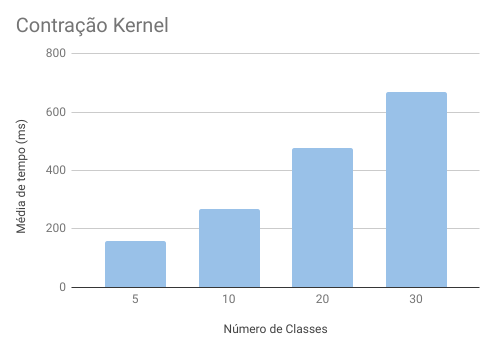
\includegraphics[width=0.6\textwidth]{Capitulos/Testes/graficock.png}
	\caption{A evolução do tempo de execução da Contração \textit{Kernel} comparada com o número de classes da ontologia.}
	\label{img:graficock}
\end{figure}

\begin{table}[H]
	\centering
	\begin{tabular}{|l|l|l|}
		\hline
		\textbf{Nº de classes}  & \textbf{Tempo médio de execução (ms)} & \textbf{Intervalo de Confiança} \\ \hline
		5                                                 & 159,096                          & {[}156,6, 161,6{]}              \\ \hline
		10                                                & 262,287                          & {[}253,3, 271,3{]}              \\ \hline
		20                                                & 477,965                          & {[}472,7, 483,2{]}              \\ \hline
		30                                                & 668,720                          & {[}663,3, 674,1{]}              \\ \hline
	\end{tabular}
	\caption{Resultados da performance da Contração \textit{Kernel} com arquivos de tamanhos diferentes.}
	\label{tab:ck}
\end{table}

\subsection{Contração \textit{Partial Meet}}

Para a Contração \textit{Partial Meet} foram utilizados os seguintes argumentos:

\begin{itemize}
	\item \texttt{-t -c --relevance -i SmallKernelWith5classes.owl -o output.owl \\ -f "A SubClassOf B1"}
	\item \texttt{-t -c --relevance -i SmallKernelWith10classes.owl -o output.owl \\ -f "A SubClassOf B1"}
	\item \texttt{-t -c --relevance -i SmallKernelWith20classes.owl -o output.owl \\ -f "A SubClassOf B1"}
	\item \texttt{-t -c --relevance -i SmallKernelWith30classes.owl -o output.owl \\ -f "A SubClassOf B1"}
\end{itemize}

Como na subseção anterior, foi gerado um gráfico, na \autoref{img:graficocpm}, que mostra a evolução do tempo de execução médio. Na \autoref{tab:cpm} estão presentes as médias e os intervalos de confiança.

\begin{figure}[H]
	\centering
	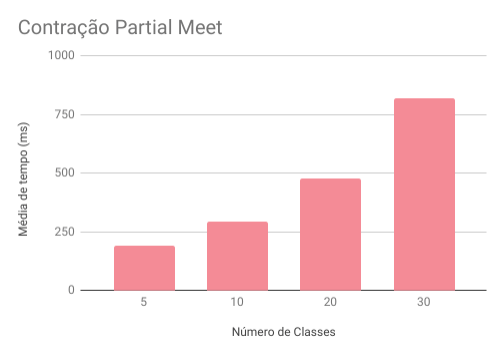
\includegraphics[width=0.6\textwidth]{Capitulos/Testes/graficocpm.png}
	\caption{A evolução do tempo de execução da Contração \textit{Partial Meet} comparada com o número de classes da ontologia.}
	\label{img:graficocpm}
\end{figure}

\begin{table}[H]
	\centering
	\begin{tabular}{|l|l|l|}
		\hline
		\textbf{Nº de classes}  & \textbf{Tempo médio de execução} & \textbf{Intervalo de Confiança} \\ \hline
		5                                                  & 190,890                          & {[}186,8, 195,0{]}              \\ \hline
		10                                                 & 294,866                          & {[}290,7, 299,0{]}              \\ \hline
		20                                                 & 476,362                          & {[}471,3, 481,4{]}              \\ \hline
		30                                                 & 818,999                          & {[}809,1, 828,9{]}              \\ \hline
	\end{tabular}
	\caption{Resultados da performance da Contração \textit{Partial Meet} com arquivos de tamanhos diferentes.}
	\label{tab:cpm}	
\end{table}

\subsection{Pseudocontração SRW}

Para a Pseudocontração SRW foram utilizados os seguintes argumentos:

\begin{itemize}
	\item \texttt{-t -srw -i SmallKernelWith5classes.owl -o output.owl -f "A SubClassOf B1"}
	\item \texttt{-t -srw -i SmallKernelWith10classes.owl -o output.owl -f "A SubClassOf B1"}
	\item \texttt{-t -srw -i SmallKernelWith20classes.owl -o output.owl -f "A SubClassOf B1"}
	\item \texttt{-t -srw -i SmallKernelWith30classes.owl -o output.owl -f "A SubClassOf B1"}
\end{itemize}

Há um gráfico, na \autoref{img:graficosrw}, que mostra a evolução do tempo de execução médio. Na \autoref{tab:srw} as médias e os intervalos de confiança podem ser vistos.

\begin{figure}[H]
	\centering
	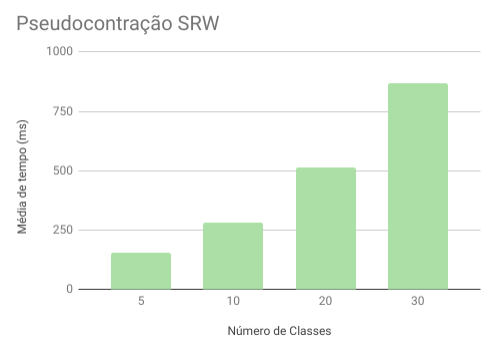
\includegraphics[width=0.6\textwidth]{Capitulos/Testes/graficosrw.png}
	\caption{A evolução do tempo de execução da Pseudocontração SRW comparada com o número de classes da ontologia.}
	\label{img:graficosrw}
\end{figure}

\begin{table}[H]
	\centering
	\begin{tabular}{|l|l|l|}
		\hline
		\textbf{Nº de classes} & \textbf{Tempo médio de execução} & \textbf{Intervalo de Confiança} \\ \hline
		5                                                 & 156,114                          & {[}153,6, 158,6{]}              \\ \hline
		10                                                & 282,843                          & {[}279,4, 286,3{]}              \\ \hline
		20                                                & 511,838                          & {[}504,8, 518,9{]}              \\ \hline
		30                                                & 867,095                          & {[}851,0, 883,2{]}              \\ \hline
	\end{tabular}
	\caption{Resultados da performance da Pseudocontração SRW com arquivos de tamanhos diferentes.}
	\label{tab:srw}
\end{table}

\subsection{Revisão \textit{Kernel}}

Para a Revisão \textit{Kernel} foram utilizados os seguintes argumentos:

\begin{itemize}
	\item \texttt{-t -r -i SmallKernelWith5classes.owl -o output.owl -f "A DisjointWith B1"}
	\item \texttt{-t -r -i SmallKernelWith10classes.owl -o output.owl -f "A DisjointWith B1"}
	\item \texttt{-t -r -i SmallKernelWith20classes.owl -o output.owl -f "A DisjointWith B1"}
	\item \texttt{-t -r -i SmallKernelWith30classes.owl -o output.owl -f "A DisjointWith B1"}
\end{itemize}

Na \autoref{img:graficork} pode ser vista a evolução do tempo de execução médio. Na \autoref{tab:rk} estão presentes as médias e os intervalos de confiança.

\begin{figure}[H]
	\centering
	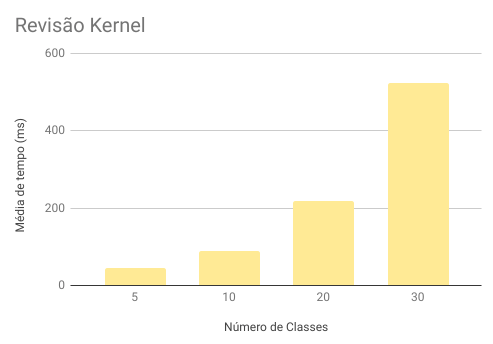
\includegraphics[width=0.6\textwidth]{Capitulos/Testes/graficork.png}
	\caption{A evolução do tempo de execução da Revisão \textit{Kernel} comparada com o número de classes da ontologia.}
	\label{img:graficork}
\end{figure}

\begin{table}[H]
	\centering
	\begin{tabular}{|l|l|l|}
		\hline
		\textbf{Nº de classes}  & \textbf{Tempo médio de execução} & \textbf{Intervalo de Confiança} \\ \hline
		5                                                  & 44,146                          & {[}42,2, 46,1{]}              \\ \hline
		10                                                  & 87,953                          & {[}85,4, 90,5{]}              \\ \hline
		20                                                  & 218,807                          & {[}215,1, 222,5{]}              \\ \hline
		30                                                 & 522,843                          & {[}516,1, 529,6{]}              \\ \hline
	\end{tabular}
	\caption{Resultados da performance da Revisão \textit{Kernel} com arquivos de tamanhos diferentes.}
	\label{tab:rk}
\end{table}

\section{Comparação}

Esses testes são, na verdade, a execução de diferentes operações sobre fórmulas próximas. O objetivo é verificar se existem diferenças nos resultados que elas fornecem. Os exemplos utilizados são bem curtos, afim de que se possa rapidamente enxergar as discrepâncias.

\subsection{Comparação das subclasses de Pessoa}

Para essa comparação, o arquivo de exemplo da \autoref{sect:srw} será revisitado, sem nenhuma alteração. Os resultados obtidos foram bem interessantes.

A execução da Contração \textit{Kernel}, com a mesma fórmula, forneceu na resposta uma estrutura de classes diferente da que veio na entrada, como pode ser visto na \autoref{fig:compckcantor1}. A classes \texttt{Cantor} e \texttt{Compositor} ficaram sem a instância, algo exibido pela \autoref{fig:compckcantor3}.

\begin{figure}[H]
	\centering
	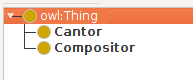
\includegraphics[width=0.3\linewidth]{Capitulos/Testes/compckcantor1}
	\caption{A estrutura de classes foi alterada.}
	\label{fig:compckcantor1}
\end{figure}

\begin{figure}[H]
	\centering
	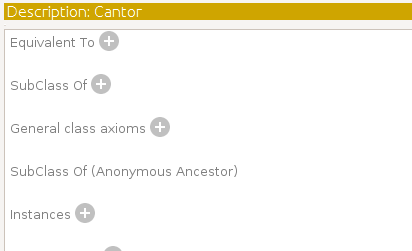
\includegraphics[width=0.44\linewidth]{Capitulos/Testes/compckcantor3}
	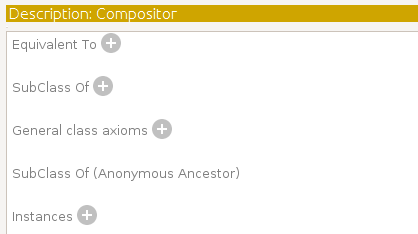
\includegraphics[width=0.48\linewidth]{Capitulos/Testes/compckcantor2}
	\caption{As classes \texttt{Cantor} e \texttt{Compositor} ficaram sem nenhuma instância.}
	\label{fig:compckcantor3}
\end{figure}

A Contração \textit{Partial Meet}, também pela mesma fórmula, tira a instância \texttt{markRonson} de ambas as classes, mas mantém a estrutura das classes. A Pseudocontração SRW, como já é sabido, também tira a instância das duas classes e altera a hierarquia das classes.

A Revisão foi feita pela fórmula \texttt{"Cantor DisjointWith Compositor"}. O resultado obtido foi idêntico ao que a Pseudocontração SRW forneceu. 

\subsection{Comparação de classes em \texttt{HinoNacional}}

Para essa comparação, foi feito um novo exemplo, com os seguintes axiomas: \texttt{MusicaBelica} $ \sqsubseteq $ \texttt{HinoNacional} e \texttt{Marcha} $ \sqsubseteq $ \texttt{MusicaBelica}. Sua hierarquia pode ser observada na \autoref{fig:comphino}. 

\begin{figure}[H]
	\centering
	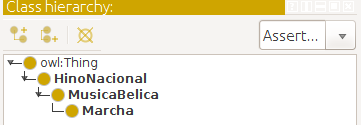
\includegraphics[width=0.5\linewidth]{Capitulos/Testes/comphino}
	\caption{A hierarquia de classes da ontologia.}
	\label{fig:comphino}
\end{figure}

As fórmulas utilizadas para a Contração \textit{Kernel}, Contração \textit{Partial Meet} e Pseudocontração SRW foram a mesma: \texttt{"Marcha SubClassOf HinoNacional"}. As operações devolveram resultados diferentes.

Tanto a Contração \textit{Kernel} quanto a Pseudocontração SRW forneceram o mesmo resultado, deixando todas as classes como irmãs, como exibido na \autoref{fig:compckhino}.

\begin{figure}[H]
	\centering
	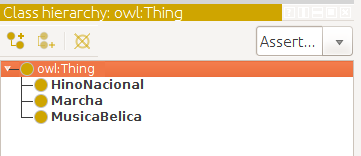
\includegraphics[width=0.5\linewidth]{Capitulos/Testes/compckhino}
	\caption{A estrutura de classes após as operações Contração \textit{Kernel} e Pseudocontração SRW.}
	\label{fig:compckhino}
\end{figure}

Já a Contração \textit{Partial Meet} fornece um resultado mais brando, mantendo o axioma \texttt{Marcha} $ \sqsubseteq $ \texttt{MusicaBelica}. Esse resultado parece ser mais promissor do que o anterior. Na \autoref{fig:compcpmhino}, é possível observar como fica a hierarquia.

\begin{figure}[H]
	\centering
	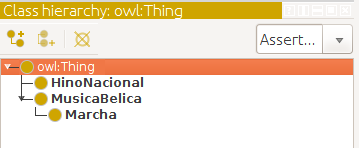
\includegraphics[width=0.5\linewidth]{Capitulos/Testes/compcpmhino}
	\caption{Hierarquia das classes após a Contração \textit{Partial Meet}.}
	\label{fig:compcpmhino}
\end{figure}

No outro oposto, temos a Revisão \textit{Kernel}. Seu resultado é o mais radical. A fórmula utilizada foi \texttt{"Marcha DisjointWith HinoNacional"}. Pode-se observar, na \autoref{fig:comprkhino}, que esse axioma está presente na ontologia, pelo postulado \textbf{Sucesso}. No entanto, os outros dois axiomas não estão mais na ontologia, e a classe \texttt{MusicaBelica} também não existe mais na estrutura. Algo semelhante havia ocorrido nos testes de performance.

\begin{figure}[H]
	\centering
	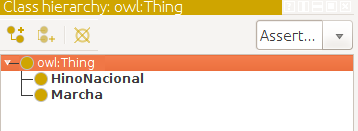
\includegraphics[width=0.5\linewidth]{Capitulos/Testes/comprkhino}
	\caption{A estrutura da ontologia, radicalmente alterada após a Revisão \textit{Kernel}.}
	\label{fig:comprkhino}
\end{figure}